% !TEX root = ../UPDATED_main.tex
Model-based phylogenetics combines tree search with branch-support measures such as the bootstrap and approximate likelihood-ratio tests \cite{felsenstein1985confidence,hoang2017,anisimova2006,minh2020iqtree}. These measures quantify the reproducibility of, or local preference for, a split. They do not test whether repeated substitutions have erased the historical dependence connecting the groups on either side of that split. A branch can therefore receive high support even when the alignment no longer contains recoverable signal across it.

Saturation is the progressive loss of historical information as multiple substitutions accumulate at the same sites \cite{philippe2011,ho2004}. Alignment-wide indices and locus filters can identify heavily saturated data \cite{xia2003index,duchene2021}, but deep phylogenies often contain mixtures of informative and uninformative genes, regions, and rate categories. A branch-specific diagnostic is needed to localize this loss.

SatuTe generalizes saturation from pairs of sequences to the two subtrees separated by a branch \cite{manuel2025satute}. Its null hypothesis is that the subtrees evolve independently. Rejection indicates detectable shared history; failure to reject classifies the branch as saturated at the selected threshold. SatuTe therefore complements branch support: branch support asks whether a split is reproducible, whereas SatuTe asks whether the alignment still connects its two sides.

For a site pattern \(\partial\), partial likelihood vectors \(L(\partial_A)\) and \(L(\partial_B)\) give the probabilities \(P(\partial_A)=\langle L(\partial_A),\pi\rangle\) and \(P(\partial_B)=\langle L(\partial_B),\pi\rangle\) for the subtrees separated by the focal branch. Under the spectral decomposition of a reversible substitution model \cite{levin2017,tavare1986}, with eigenvalues \(\lambda_0=0>\lambda_1\geq\lambda_2\geq\cdots\) and left eigenvectors \(h_i\), the coherence coefficient is
\begin{equation}
C_{\partial i}
=
\left\langle \frac{L(\partial_A)}{P(\partial_A)},h_i\right\rangle
\left\langle \frac{L(\partial_B)}{P(\partial_B)},h_i\right\rangle .
\label{eq-coherence}
\end{equation}
Original SatuTe retains the slowest non-stationary component. This published formulation remains the reference test throughout our analyses.

We first reproduce the original Jukes--Cantor (JC) design and use it to distinguish branch support from recoverable historical signal. We then ask whether faster spectral components should contribute while they persist on a finite branch and derive weights from their decay relative to the slowest component. We also correct the infinite-branch null for explicit invariant sites, which retain ancestral dependence even as the focal branch tends to infinity. Both changes preserve the branch-specific question posed by SatuTe rather than define a different primary model.

We evaluate these extensions in paired nucleotide and protein simulations under three decision rules and in independent truth-labeled calibration experiments. Finally, we apply original and extended SatuTe analyses to ribosomal-protein two-domain and 16S rRNA three-domain Tree-of-Life examples \cite{hug2016,williams2D,woese1990}, and to codon-position partitions from a hepatitis C virus reference panel. These applications are designed to identify branches and alignment regions that retain detectable signal under a fitted model, not to select a Tree-of-Life topology or infer viral population structure.

\begin{figure}[p]
  \vspace*{-2.4cm}
  \centering
  \makebox[\textwidth][c]{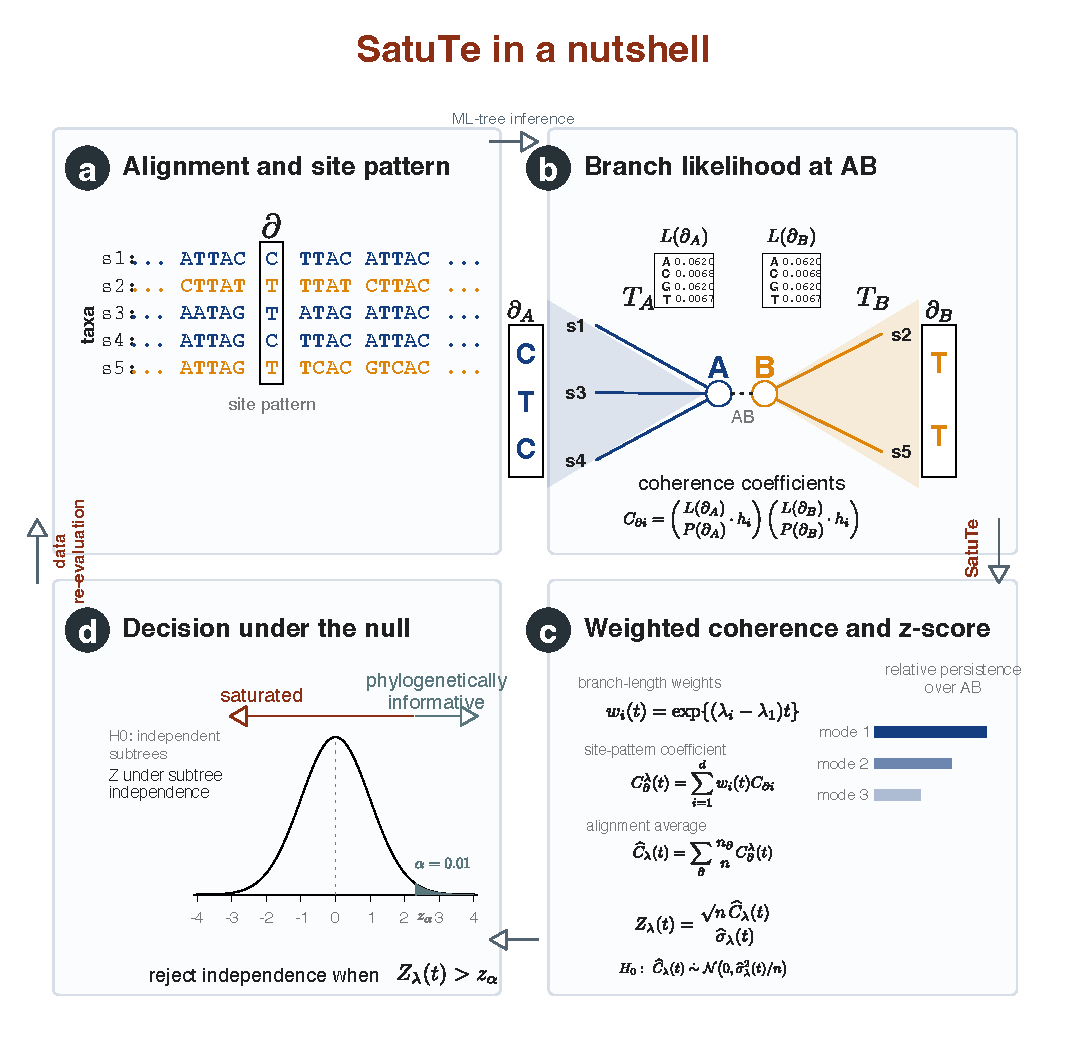
\includegraphics[width=1.10\textwidth]{figures/figure1_satute_weighted_workflow.pdf}}
  \caption{\textbf{Branch-specific detection of phylogenetic signal with SatuTe.} \textbf{a,} Columns of a five-taxon alignment define site patterns \(\partial\). \textbf{b,} The focal branch partitions each pattern into two subtree patterns used to calculate partial likelihoods and coherence coefficients. \textbf{c,} Original SatuTe uses the slowest non-stationary component; the model-aware extension weights additional components by their persistence relative to that reference over branch length \(t\). \textbf{d,} Rejection of subtree independence indicates detectable signal, whereas failure to reject indicates saturation at the selected threshold.}
  \makeatletter\cref@old@label{fig-workflow}\makeatother
\end{figure}
